\documentclass[a4paper,11pt]{article}
\usepackage{latexsym,amssymb,enumerate,amsmath,epsfig,amsthm}
\usepackage[margin=1in]{geometry}
\usepackage{setspace,color}
\usepackage{graphics}
\usepackage{subfigure}
\usepackage{hyperref}
\usepackage{subfiles} 
\usepackage{float}

\newcommand{\redcolor}[1]{\textcolor{red}{#1}}
\graphicspath{ {./images/} }



%\newcommand{\x}{\mathbf{x}}
%\newcommand{\y}{\mathbf{y}}
%\newcommand{\bv}{\mathbf{v}}
%\newcommand{\n}{\mathbf{n}}
%\newcommand{\colored}[1]{\textcolor{red}{#1}}
%\newtheorem{thm}{Theorem}[section]
%\newtheorem{prop}{Proposition}[section]
%\newtheorem{obser}{Observation}[section]
%\newtheorem{corollary}{Corollary}[section]

%\doublespacing

\title{Blind Source Separation of Stereo Mixtures Using Wavelet Transform}
\author{
CHOI, Seung-ryeol \thanks{Department of Mathematics, the Hong Kong University of Science and Technology, Clear Water Bay, Hong Kong. Email: {\bf schoiak@connect.ust.hk}}
\and
KIM, Minji \thanks{Department of Mathematics, the Hong Kong University of Science and Technology, Clear Water Bay, Hong Kong. Email: {\bf mkimao@connect.ust.hk}}  
}

\markboth{First author}{MATH4992 Project Final Report}
\pagestyle{myheadings}
\date{30 November 2022}

\begin{document}
\thispagestyle{plain}
\maketitle


\begin{abstract}
Blind Source Separation refers to a problem where the independent sources should be separated from the set of measurements without or with little information about the sources or the mixing process. It is often challenging when the situation is underdetermined i.e. the number of sources is more than the number of measurements. In this project, we will investigate an approach for solving the Blind Source Separation Problem with the assumption that the source signals have sparse approximation supports.
\end{abstract}

\section{Introduction}

\subsection{Background}
Blind Source Separation problem is a well-known signal processing problem where the independent sources should be separated from the mixture of signals. An example is separating the sounds of K musical instruments from P microphones recordings without knowing the original sources and their mixing parameters.
\\ \\
\noindent A linear model is appropriate for representing a mixture of sound sources. The P channel measurement of K sources can be written as,

\begin{equation}
    y_p[n] = \sum \limits _{{k=1 }}^{K}{m_{p,k}}{s_k[n]} + \epsilon_k[n], \;for \;   1\leqslant{p}\leqslant{P} \;
\end{equation}

\noindent where $ M = \{m_{p,k}\}_{1\leq p \leq P, 1\leq k \leq K} $ is the mixing matrix and $\epsilon_k[n]$ are measurement noise.
\\

\noindent The number of K sources is unknown, and it is often greater than the number of measurements P which makes the problem underdetermined. Thus, knowing the mixing matrix M is not enough to recover the sources $s_k$ from the measurement $y_p$.
In this paper, we will introduce a successful method for source separation under the condition that sources have sparse approximation supports.


\subsection{Blind Source Separation}
Blind source separation is a fundamental of signal processing that has received a great amount of attention recently. Recently, many researchers have explored a number of techniques to solve the blind source separation problem\cite{1576973}\cite{ica}\cite{6025435}. One effective source separation method is based on stochastic models, where the sources must be independent\cite{COMON1994287}. However, it can be challenging to formulate a stochastic model of complicated signals and hence confirm their independence. \\
\\
\noindent Instead, we will use a method that is based on weaker deterministic models.
Jourjine, Rickard, and Yilmaz as well as Zibulevsky et al introduced an algorithm called Sparse Blind Source Separation, which estimates the mixing parameters under the assumption that the source supports do not overlap too much in an appropriate domain.\cite{1461442}\cite{BOFILL20012353}



\subsection{Project Objective}
In this paper, we aim to achieve two main project objectives:\\
\indent 1. Estimating the mixing matrix \textbf{\textit{M}} \\
\indent 2. Separating independent $\boldsymbol{S}$ sources from the measurements $\boldsymbol{y_p[n]}$. 



\section{Methodology}

\subsection{Multi-level Discrete Wavelet Transform}
For blind source separation, the mixing parameters $m_{p,k}$ can be estimated by defining a dictionary where different sources have a sparse representation. Here, we will use a Multi-level Discrete Wavelet Transform to obtain such a dictionary.\\
\\
Multi-level Discrete Wavelet Transform decomposes signals into a shifted and scaled versions of the basis wavelet. At different dilatation, wavelet coefficients can be obtained that represent various levels of frequencies. As we can observe from Figure 1, smaller scales i.e., lower-level wavelet transform, are associated with high frequencies, whereas larger scales are associated with the low-frequency information. Since high-frequency components are a complement to low-frequency components, wavelet coefficients then can be our dictionary that has a sparse representation.


\begin{figure}[H]
    \centering
    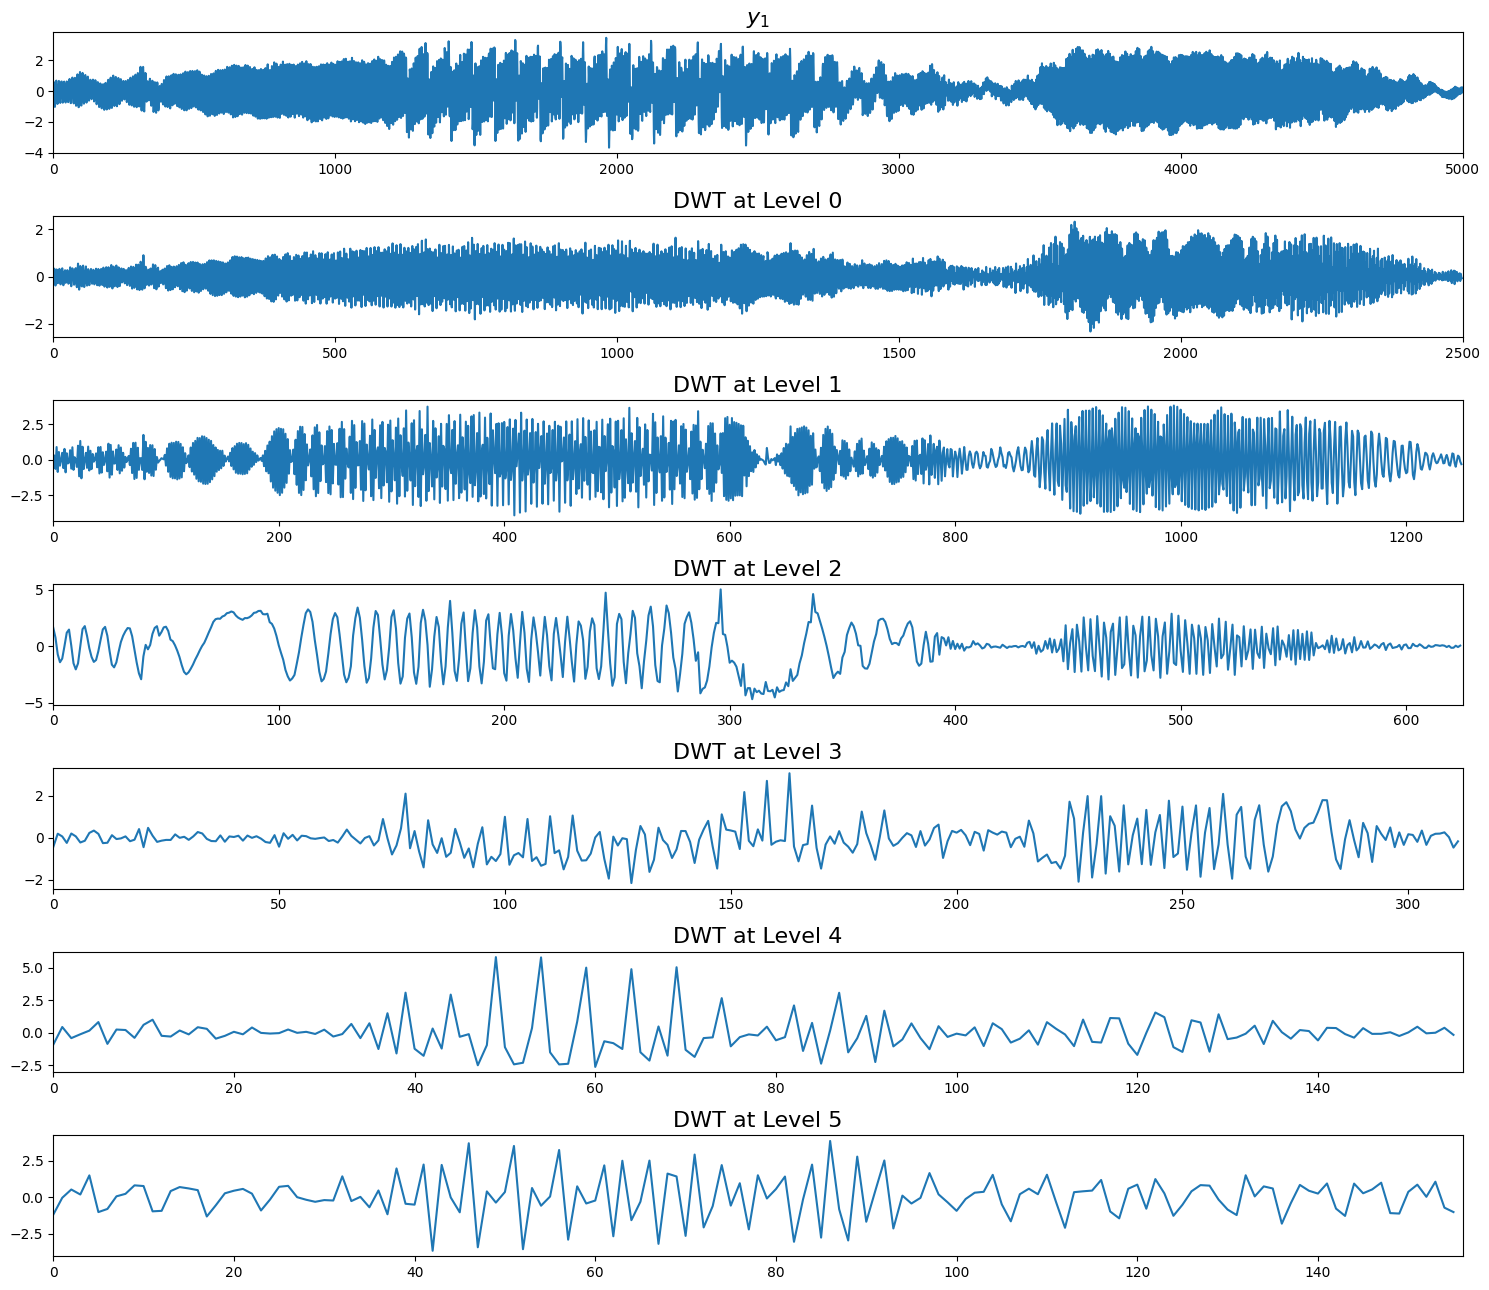
\includegraphics[width=0.65\linewidth]{sources/wt.png}
    \caption{\textbf{(a)} Multi-level Discrete Wavelet Transform of $y_1$}
    \label{fig:my_label}
\end{figure}



\subsection{Assumption}
Sparse blind source separation requires constrained condition i.e., the source supports directions are distinct. In order to fulfill the constrained condition, We assume that no two mixing directions are parallel such that,
\begin{equation}
\vec{m}_{\,a} \neq k\vec{m}_{\,b}, for \ some \ \vec{m}_a, \ \vec{m}_b \in M, a \neq b
\end{equation} 
where $k$ is some constant in $\mathbb{R}$.\\
\\
In addition, for the simplicity of the experiment formulation we assume that the noise term $\epsilon_p$ is negligible such that,
\begin{equation}
    \epsilon_p = 0, \quad \text{for} \; 1\leq p \leq P
\end{equation}
which makes our measurement equation $y_p[n]$ as below:
\begin{equation}
    y_p[n] = \sum \limits _{{k=1 }}^{K}{m_{p,k}}{s_k[n]}, \;for \;   1\leqslant{p}\leqslant{P} \;
\end{equation}


\subsection{Data Preprocessing}
Before we begin our experiment, we will simulate the stereo channel measurement of 3 sound sources which are the bird, male and female sounds accordingly. We will first construct a mixing matrix M, which will be the ground truth mixing parameters. The measurements $y_n$, then can be obtained by taking the inner product of the original sources and the mixing matrix.
To ensure the data uniformity, we used normalized sources.\\
\\
Since the source supports of $s_k[n]$ should have distinct directions we have set the mixing matrix using trigonometry in such a way that,
\begin{equation}
M = 
\begin{bmatrix}m_{1,1}&m_{1,2}&m_{1,3}\\
m_{2,1}&m_{2,2}&m_{2,3}
\end{bmatrix}
= \begin{bmatrix}\cos(\theta_1)&\cos(\theta_2)&\cos(\theta_3)\\
\sin(\theta_1)&\sin(\theta_2)&\sin(\theta_3)
\end{bmatrix}
\end{equation}
\[
\text{where} \quad
\theta_{k} \neq \theta_{k^{'}}\; \text{and} \; k \neq k^{'} \; \text{for} \;\; k, k^{'} \in \{1, 2, 3\}
\]
\\
Then we will take the inner product of the sources and the mixing matrix.
\begin{equation}
    Y = \binom{y_1[n]}{y_2[n]}  = \langle M, S \rangle
\end{equation}
In the other words, we obtained the measurements that are the linear combinations of the original source signals with mixing parameters $m_{p,k}$.

\begin{equation}
\begin{split}
    y_1[n] & = m_{1,1}s_1[n] + m_{1,2}s_2[n] +m_{1,3}s_3[n] \\
    y_2[n] & = m_{2,1}s_1[n] + m_{2,2}s_2[n] +m_{2,3}s_3[n]
\end{split}
\end{equation}
\\

\begin{figure}[H]
\centering
\subfigure[]{
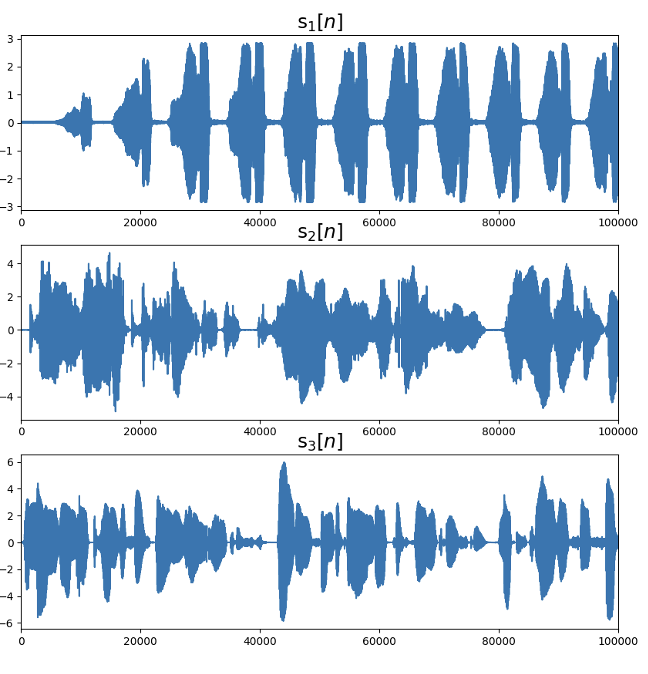
\includegraphics[width=0.35\linewidth]{sources/s.png}
}
\centering
\subfigure[]{
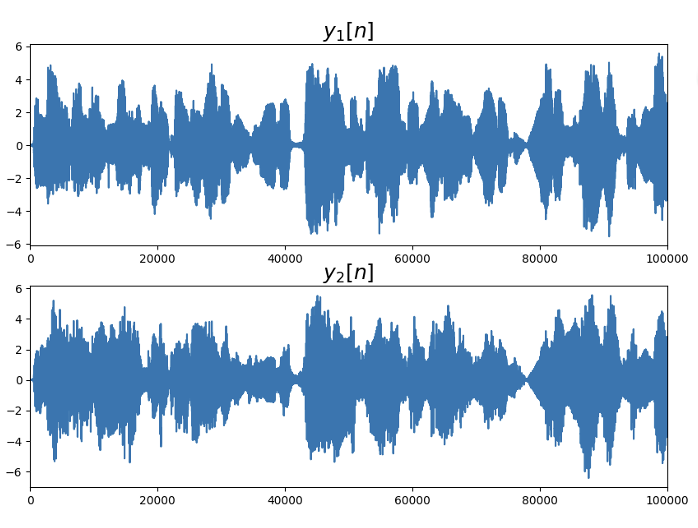
\includegraphics[width=0.35\linewidth]{sources/y.png}
}
\caption{\textbf{(a)} source signals $s_1[n]$, $s_2[n]$, and $s_3[n]$ \; \textbf{(b)} mixture of sources $y_1[n]$ and $y_2[n]$}
\label{fig:long}
\label{fig:onecol}
\end{figure}

\noindent From now on, we will only use the measurements $y_1[n]$ and $y_2[n]$ to recover the original sources $s_1[n]$, $s_2[n]$, and $s_3[n]$ without knowing the mixing parameters.


\end{document}
